\documentclass[]{article}
\usepackage{lmodern}
\usepackage{amssymb,amsmath}
\usepackage{ifxetex,ifluatex}
\usepackage{fixltx2e} % provides \textsubscript
\ifnum 0\ifxetex 1\fi\ifluatex 1\fi=0 % if pdftex
  \usepackage[T1]{fontenc}
  \usepackage[utf8]{inputenc}
\else % if luatex or xelatex
  \ifxetex
    \usepackage{mathspec}
    \usepackage{xltxtra,xunicode}
  \else
    \usepackage{fontspec}
  \fi
  \defaultfontfeatures{Mapping=tex-text,Scale=MatchLowercase}
  \newcommand{\euro}{€}
\fi
% use upquote if available, for straight quotes in verbatim environments
\IfFileExists{upquote.sty}{\usepackage{upquote}}{}
% use microtype if available
\IfFileExists{microtype.sty}{%
\usepackage{microtype}
\UseMicrotypeSet[protrusion]{basicmath} % disable protrusion for tt fonts
}{}
\usepackage[margin=1in]{geometry}
\usepackage{color}
\usepackage{fancyvrb}
\newcommand{\VerbBar}{|}
\newcommand{\VERB}{\Verb[commandchars=\\\{\}]}
\DefineVerbatimEnvironment{Highlighting}{Verbatim}{commandchars=\\\{\}}
% Add ',fontsize=\small' for more characters per line
\usepackage{framed}
\definecolor{shadecolor}{RGB}{248,248,248}
\newenvironment{Shaded}{\begin{snugshade}}{\end{snugshade}}
\newcommand{\KeywordTok}[1]{\textcolor[rgb]{0.13,0.29,0.53}{\textbf{{#1}}}}
\newcommand{\DataTypeTok}[1]{\textcolor[rgb]{0.13,0.29,0.53}{{#1}}}
\newcommand{\DecValTok}[1]{\textcolor[rgb]{0.00,0.00,0.81}{{#1}}}
\newcommand{\BaseNTok}[1]{\textcolor[rgb]{0.00,0.00,0.81}{{#1}}}
\newcommand{\FloatTok}[1]{\textcolor[rgb]{0.00,0.00,0.81}{{#1}}}
\newcommand{\CharTok}[1]{\textcolor[rgb]{0.31,0.60,0.02}{{#1}}}
\newcommand{\StringTok}[1]{\textcolor[rgb]{0.31,0.60,0.02}{{#1}}}
\newcommand{\CommentTok}[1]{\textcolor[rgb]{0.56,0.35,0.01}{\textit{{#1}}}}
\newcommand{\OtherTok}[1]{\textcolor[rgb]{0.56,0.35,0.01}{{#1}}}
\newcommand{\AlertTok}[1]{\textcolor[rgb]{0.94,0.16,0.16}{{#1}}}
\newcommand{\FunctionTok}[1]{\textcolor[rgb]{0.00,0.00,0.00}{{#1}}}
\newcommand{\RegionMarkerTok}[1]{{#1}}
\newcommand{\ErrorTok}[1]{\textbf{{#1}}}
\newcommand{\NormalTok}[1]{{#1}}
\usepackage{graphicx}
\makeatletter
\def\maxwidth{\ifdim\Gin@nat@width>\linewidth\linewidth\else\Gin@nat@width\fi}
\def\maxheight{\ifdim\Gin@nat@height>\textheight\textheight\else\Gin@nat@height\fi}
\makeatother
% Scale images if necessary, so that they will not overflow the page
% margins by default, and it is still possible to overwrite the defaults
% using explicit options in \includegraphics[width, height, ...]{}
\setkeys{Gin}{width=\maxwidth,height=\maxheight,keepaspectratio}
\ifxetex
  \usepackage[setpagesize=false, % page size defined by xetex
              unicode=false, % unicode breaks when used with xetex
              xetex]{hyperref}
\else
  \usepackage[unicode=true]{hyperref}
\fi
\hypersetup{breaklinks=true,
            bookmarks=true,
            pdfauthor={},
            pdftitle={NRGFigs},
            colorlinks=true,
            citecolor=blue,
            urlcolor=blue,
            linkcolor=magenta,
            pdfborder={0 0 0}}
\urlstyle{same}  % don't use monospace font for urls
\setlength{\parindent}{0pt}
\setlength{\parskip}{6pt plus 2pt minus 1pt}
\setlength{\emergencystretch}{3em}  % prevent overfull lines
\setcounter{secnumdepth}{0}

%%% Use protect on footnotes to avoid problems with footnotes in titles
\let\rmarkdownfootnote\footnote%
\def\footnote{\protect\rmarkdownfootnote}

%%% Change title format to be more compact
\usepackage{titling}
\setlength{\droptitle}{-2em}
  \title{NRGFigs}
  \pretitle{\vspace{\droptitle}\centering\huge}
  \posttitle{\par}
  \author{}
  \preauthor{}\postauthor{}
  \date{}
  \predate{}\postdate{}




\begin{document}

\maketitle


\begin{Shaded}
\begin{Highlighting}[]
\KeywordTok{library}\NormalTok{(knitr)}
\KeywordTok{library}\NormalTok{(ggplot2)}
\KeywordTok{library}\NormalTok{(dplyr)}
\KeywordTok{library}\NormalTok{(tidyr)}
\KeywordTok{library}\NormalTok{(xtable)}
\NormalTok{filename<-}\StringTok{"~/MATLAB/NeurophysNRG/bestFitLRResort.csv"}
\NormalTok{d <-}\StringTok{ }\KeywordTok{read.csv}\NormalTok{(filename, }\DataTypeTok{na.strings=}\StringTok{"NaN"}\NormalTok{)}
\NormalTok{r<-}\KeywordTok{read.csv}\NormalTok{(}\StringTok{'peakregressions.csv'}\NormalTok{)}
\NormalTok{gs<-}\KeywordTok{read.csv}\NormalTok{(}\StringTok{'~/MATLAB/NeurophysNRG/fitGSPlm.csv'}\NormalTok{)}
\NormalTok{r<-r[,}\DecValTok{2}\NormalTok{:}\DecValTok{12}\NormalTok{]}
\end{Highlighting}
\end{Shaded}

\begin{Shaded}
\begin{Highlighting}[]
\NormalTok{ptab<-}\KeywordTok{subset}\NormalTok{(d,d$rsquared>}\DecValTok{0}\NormalTok{)}
\NormalTok{tab<-}\KeywordTok{xtable}\NormalTok{(ptab[,}\DecValTok{1}\NormalTok{:}\DecValTok{4}\NormalTok{],}\DataTypeTok{caption=}\StringTok{'This table shows the results of a step-wise fitting procedure that with a threshold for inclusion of an increase of 0.5 in the R2'}\NormalTok{)}
\KeywordTok{print}\NormalTok{(tab,}\DataTypeTok{comment=}\OtherTok{FALSE}\NormalTok{)}
\end{Highlighting}
\end{Shaded}

\begin{table}[ht]
\centering
\begin{tabular}{rlrrl}
  \hline
 & Neuron & shift & rsquared & f \\ 
  \hline
1 & SB21Oct11 & 120 & 0.77 & fr \~{} 1 + rhv + rep \\ 
  2 & UB21dec11 &  60 & 0.70 & fr \~{} 1 + lep \\ 
  3 & UB22may12 &  70 & 0.64 & fr \~{} 1 + rhv + lhv \\ 
  4 & SE17Oct11 & 150 & 0.58 & fr \~{} 1 + rhv \\ 
  5 & SB10Oct11 & 170 & 0.58 & fr \~{} 1 + rhp + rhv \\ 
  6 & UC22may12 &  80 & 0.57 & fr \~{} 1 + rhv + lhv \\ 
  7 & SC23Sep11 & 130 & 0.47 & fr \~{} 1 + lhv \\ 
  8 & UBA4jun12 &  90 & 0.46 & fr \~{} 1 + rhv + lhv \\ 
  9 & SD09Jan12 & 130 & 0.41 & fr \~{} 1 + lhv \\ 
  10 & UB23mar12 &  80 & 0.40 & fr \~{} 1 + lhv + rep \\ 
  11 & SC12Dec11 &  70 & 0.40 & fr \~{} 1 + lhv \\ 
  12 & UB16feb12 &  90 & 0.40 & fr \~{} 1 + lhv \\ 
  13 & UB05jan12 &  60 & 0.39 & fr \~{} 1 + lhp + lhv + rha \\ 
  14 & SB15Sep11 & 110 & 0.37 & fr \~{} 1 + rhv \\ 
  15 & UB28sep11 &  20 & 0.35 & fr \~{} 1 + rhp + rhv + rep \\ 
  16 & SD03Nov11 & 160 & 0.34 & fr \~{} 1 + lhv \\ 
  17 & SC18Oct11 &  40 & 0.33 & fr \~{} 1 + rhv + lep \\ 
  18 & SB16Sep11 &  70 & 0.32 & fr \~{} 1 + lhv \\ 
  19 & UD16sep11 & 130 & 0.32 & fr \~{} 1 + lhv \\ 
  20 & UB04nov11 &  70 & 0.31 & fr \~{} 1 + rhv + lhv \\ 
  21 & UBB4jun12 & 130 & 0.30 & fr \~{} 1 + rhv + lhv \\ 
  22 & SB18Oct11 &  70 & 0.30 & fr \~{} 1 + rhv \\ 
  23 & UB26mar12 &  80 & 0.30 & fr \~{} 1 + lhv \\ 
  24 & UE31oct11 &  40 & 0.29 & fr \~{} 1 + rhv + lhv \\ 
  25 & SC21Dec11 & 130 & 0.29 & fr \~{} 1 + lhv \\ 
  26 & SC07Oct11 &  80 & 0.28 & fr \~{} 1 + lhp + lhv \\ 
  27 & SD13Jan12 & 190 & 0.27 & fr \~{} 1 + lhv \\ 
  28 & UC17feb12 & 100 & 0.26 & fr \~{} 1 + lhv + rep \\ 
  29 & SC16Sep11 &  60 & 0.26 & fr \~{} 1 + lhv + lep \\ 
  30 & UB24oct11 &  50 & 0.24 & fr \~{} 1 + rhv \\ 
  31 & UC03jan12 & 110 & 0.23 & fr \~{} 1 + lhv + rep \\ 
  32 & UB14may12 & 100 & 0.23 & fr \~{} 1 + rhv + lhv \\ 
  33 & SC19Oct11 &  70 & 0.22 & fr \~{} 1 + rhv \\ 
  34 & SD30Sep11 & 200 & 0.22 & fr \~{} 1 + rhp + rhv \\ 
  35 & SC28Nov11 & 110 & 0.21 & fr \~{} 1 + lhv + lep \\ 
  36 & SC14Oct11 & 180 & 0.20 & fr \~{} 1 + rhv \\ 
  37 & SD04Jan12 &  60 & 0.20 & fr \~{} 1 + rhv \\ 
  38 & SC19Jan12 & 190 & 0.20 & fr \~{} 1 + lhv \\ 
  39 & SB28Sep11 &  50 & 0.19 & fr \~{} 1 + rhv + lep \\ 
  40 & SD21Sep11 &  60 & 0.18 & fr \~{} 1 + rhv + lhv \\ 
  41 & SB05Oct11 &  80 & 0.17 & fr \~{} 1 + rhv + lhv \\ 
  42 & SB10Jan12 &  90 & 0.17 & fr \~{} 1 + lhv + lep \\ 
  43 & SB30Sep11 & 130 & 0.16 & fr \~{} 1 + rhv \\ 
  44 & SB19Jan12 & 120 & 0.16 & fr \~{} 1 + rhv \\ 
  45 & SD06Dec11 &  50 & 0.15 & fr \~{} 1 + rhv + lhv \\ 
  46 & SB04Nov11 &  90 & 0.15 & fr \~{} 1 + rhv + lhv \\ 
  47 & UB07oct11 &  80 & 0.14 & fr \~{} 1 + lhp + rhv \\ 
  48 & UB23feb12 &  50 & 0.13 & fr \~{} 1 + rhv \\ 
  49 & SD28Sep11 & 130 & 0.09 & fr \~{} 1 + rep \\ 
  50 & UB11jan12 &  40 & 0.06 & fr \~{} 1 + lhp \\ 
  51 & SB07Oct11 & 200 & 0.05 & fr \~{} 1 + rhv \\ 
   \hline
\end{tabular}
\caption{This table shows the results of a step-wise fitting procedure that with a threshold for inclusion of an increase of 0.5 in the R2} 
\end{table}

\begin{Shaded}
\begin{Highlighting}[]
\NormalTok{s<-d %>%}\StringTok{ }
\StringTok{  }\KeywordTok{select}\NormalTok{(rhv:lea) %>%}\StringTok{ }
\StringTok{  }\KeywordTok{mutate_each}\NormalTok{(}\KeywordTok{funs}\NormalTok{(!}\KeywordTok{is.na}\NormalTok{(.))) %>%}
\StringTok{  }\KeywordTok{summarise_each}\NormalTok{(}\KeywordTok{funs}\NormalTok{(sum)) %>%}\StringTok{ }
\StringTok{  }\KeywordTok{gather}\NormalTok{(}\StringTok{'c'}\NormalTok{,}\StringTok{'n'}\NormalTok{,}\DecValTok{1}\NormalTok{:}\DecValTok{12}\NormalTok{) %>%}
\StringTok{  }\KeywordTok{mutate}\NormalTok{(}\DataTypeTok{c=}\KeywordTok{reorder}\NormalTok{(c,}\KeywordTok{desc}\NormalTok{(n)))}

\NormalTok{p<-}\KeywordTok{ggplot}\NormalTok{(}\KeywordTok{aes}\NormalTok{(}\DataTypeTok{y=}\NormalTok{n),}\DataTypeTok{data=}\NormalTok{s)+}\KeywordTok{theme}\NormalTok{(}\DataTypeTok{axis.text.x=}\KeywordTok{element_text}\NormalTok{(}\DataTypeTok{size=}\DecValTok{18}\NormalTok{,}\DataTypeTok{angle=}\DecValTok{45}\NormalTok{, }\DataTypeTok{hjust=}\DecValTok{1}\NormalTok{))}
\NormalTok{p+}\KeywordTok{geom_bar}\NormalTok{(}\KeywordTok{aes}\NormalTok{(}\DataTypeTok{x=}\NormalTok{s$c),}\DataTypeTok{stat=}\StringTok{'identity'}\NormalTok{)+}\KeywordTok{xlab}\NormalTok{(}\StringTok{'Coefficient'}\NormalTok{)+}\KeywordTok{ylab}\NormalTok{(}\StringTok{'Count'}\NormalTok{)}
\end{Highlighting}
\end{Shaded}

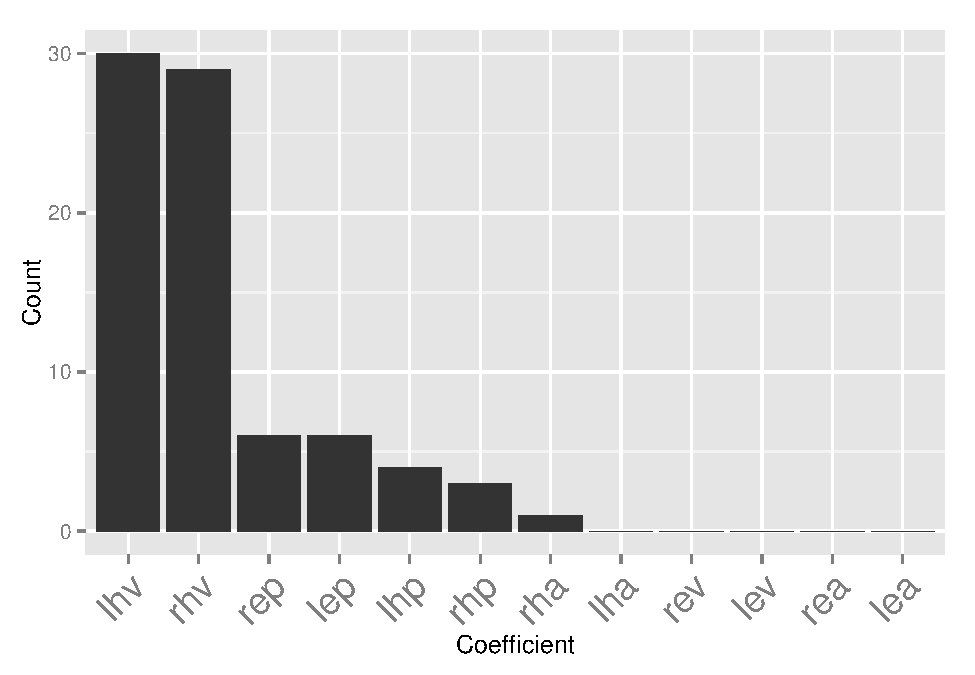
\includegraphics{ExtraFigs_files/figure-latex/coefCounts-1.pdf}

\begin{Shaded}
\begin{Highlighting}[]
\NormalTok{staticBestFitLR <-}\StringTok{ }\KeywordTok{read.csv}\NormalTok{(}\StringTok{"~/MATLAB/NeurophysNRG/Resort/staticBestFitLR.csv"}\NormalTok{, }\DataTypeTok{na.strings=}\StringTok{"NaN"}\NormalTok{)}

\NormalTok{staticBestFitLR %>%}
\StringTok{  }\KeywordTok{select}\NormalTok{(}\DecValTok{1}\NormalTok{:}\DecValTok{6}\NormalTok{) %>%}
\StringTok{  }\KeywordTok{rename}\NormalTok{(}\DataTypeTok{Rightward.Eye=}\NormalTok{rep,}\DataTypeTok{Leftward.Eye=}\NormalTok{lep,}\DataTypeTok{Rightward.Head=}\NormalTok{rhp) %>%}
\StringTok{  }\KeywordTok{gather}\NormalTok{(}\StringTok{'coef'}\NormalTok{,}\StringTok{'b'}\NormalTok{,}\DecValTok{4}\NormalTok{:}\DecValTok{6}\NormalTok{) %>%}
\StringTok{  }\KeywordTok{group_by}\NormalTok{(Neuron) %>%}
\StringTok{  }\KeywordTok{summarise}\NormalTok{(}\DataTypeTok{Coef=}\KeywordTok{max}\NormalTok{(b),}\DataTypeTok{Position.Type=}\NormalTok{coef[b==Coef]) %>%}
\StringTok{  }\KeywordTok{arrange}\NormalTok{(}\KeywordTok{desc}\NormalTok{(Coef))->}\StringTok{ }\NormalTok{t}
\NormalTok{caption.static<-}\StringTok{'Coefficient of Static Acitivy. This table shows the fit value for the position parameter that provided the greatest contribution to the model fr ~ rhp+lhp+rep+lep. Only cells that included a position parameter in the stepwise fit outcome are included.'}
\NormalTok{static.table<-}\KeywordTok{xtable}\NormalTok{(t)}
\KeywordTok{print}\NormalTok{(static.table,}\DataTypeTok{comment=}\OtherTok{FALSE}\NormalTok{)}
\end{Highlighting}
\end{Shaded}

\begin{table}[ht]
\centering
\begin{tabular}{rlrl}
  \hline
 & Neuron & Coef & Position.Type \\ 
  \hline
1 & UB21dec11 & 7.97 & Leftward.Eye \\ 
  2 & SB28Sep11 & 2.49 & Rightward.Head \\ 
  3 & SB21Oct11 & 2.07 & Rightward.Eye \\ 
  4 & SC18Oct11 & 1.11 & Rightward.Head \\ 
  5 & SB10Oct11 & 0.97 & Rightward.Eye \\ 
  6 & SC28Nov11 & 0.95 & Rightward.Eye \\ 
  7 & UB05jan12 & 0.87 & Rightward.Head \\ 
  8 & SC16Sep11 & 0.74 & Rightward.Eye \\ 
  9 & UB28sep11 & 0.69 & Rightward.Head \\ 
  10 & SC07Oct11 & 0.48 & Rightward.Head \\ 
  11 & UC17feb12 & 0.47 & Rightward.Head \\ 
  12 & UC03jan12 & 0.44 & Rightward.Eye \\ 
  13 & UB23mar12 & 0.40 & Rightward.Head \\ 
   \hline
\end{tabular}
\end{table}

\begin{Shaded}
\begin{Highlighting}[]
\NormalTok{g<-}\KeywordTok{subset}\NormalTok{(gs,rsquared>}\DecValTok{0}\NormalTok{) }\CommentTok{#gs loaded in first chunk}
\NormalTok{tall<-g %>%}\StringTok{ }\KeywordTok{gather}\NormalTok{(key,value,}\KeywordTok{c}\NormalTok{(}\DecValTok{6}\NormalTok{,}\DecValTok{7}\NormalTok{,}\DecValTok{8}\NormalTok{,}\DecValTok{9}\NormalTok{,}\DecValTok{10}\NormalTok{,}\DecValTok{12}\NormalTok{))}

\CommentTok{#tall$key<-factor(tall$key,levels=c('rhv','lhv','rep','lep','rhp','rha'))}
\CommentTok{#qplot(value,facets=key~.,data=tall,fill=tall$gsp,binwidth=0.1)+scale_fill_discrete(name="Trial\textbackslash{}nType")}

\NormalTok{tall<-g %>%}\StringTok{ }\KeywordTok{gather}\NormalTok{(key,value,}\KeywordTok{c}\NormalTok{(}\DecValTok{6}\NormalTok{,}\DecValTok{7}\NormalTok{))}
\CommentTok{#qplot(value,facets=key~.,data=tall,fill=tall$gsp,binwidth=0.1)+scale_fill_discrete(name="Trial\textbackslash{}nType")}

\KeywordTok{qplot}\NormalTok{(key,value,}\DataTypeTok{data=}\NormalTok{tall,}\DataTypeTok{geom=}\StringTok{'boxplot'}\NormalTok{,}\DataTypeTok{fill=}\NormalTok{gsp)+}
\StringTok{  }\KeywordTok{scale_fill_grey}\NormalTok{(}\DataTypeTok{start=}\DecValTok{0}\NormalTok{)+}
\StringTok{  }\KeywordTok{theme_bw}\NormalTok{()+}
\StringTok{  }\KeywordTok{theme}\NormalTok{(}\DataTypeTok{legend.position =} \StringTok{"bottom"}\NormalTok{)}
\end{Highlighting}
\end{Shaded}

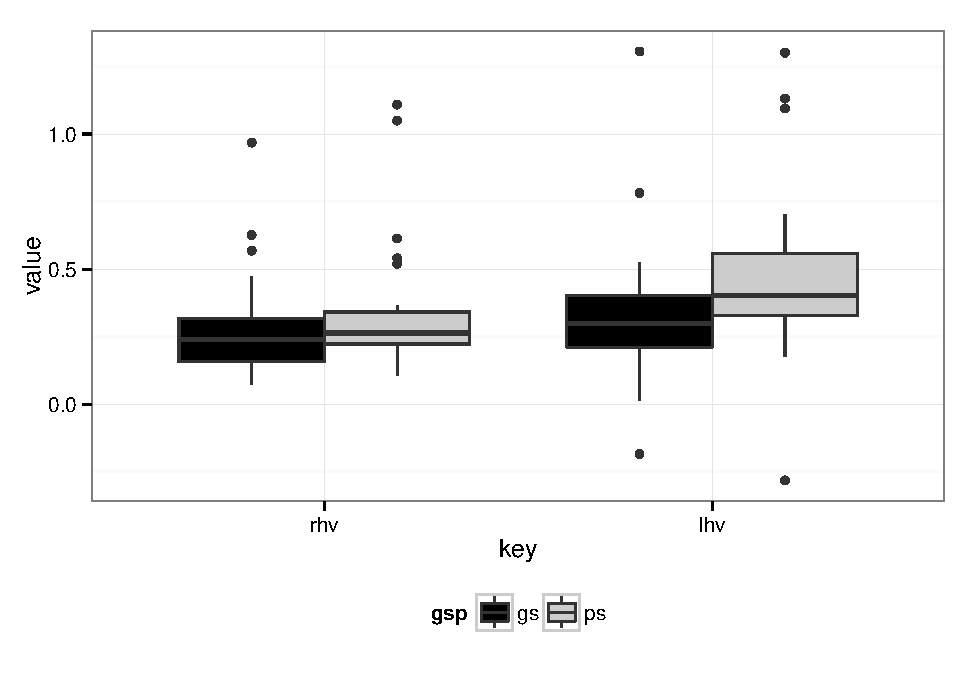
\includegraphics{ExtraFigs_files/figure-latex/gspdiff-1.pdf}

\begin{Shaded}
\begin{Highlighting}[]
\NormalTok{g %>%}\StringTok{ }
\StringTok{  }\KeywordTok{select}\NormalTok{(}\DecValTok{1}\NormalTok{,}\DecValTok{5}\NormalTok{,}\DecValTok{6}\NormalTok{) %>%}\StringTok{ }
\StringTok{  }\KeywordTok{spread}\NormalTok{(gsp,rhv) %>%}\StringTok{ }
\StringTok{  }\KeywordTok{mutate}\NormalTok{(}\DataTypeTok{rhv=}\NormalTok{ps-gs)->}\StringTok{ }\NormalTok{rdiff}
\NormalTok{g %>%}\StringTok{ }
\StringTok{  }\KeywordTok{select}\NormalTok{(}\DecValTok{1}\NormalTok{,}\DecValTok{5}\NormalTok{,}\DecValTok{7}\NormalTok{) %>%}\StringTok{ }
\StringTok{  }\KeywordTok{spread}\NormalTok{(gsp,lhv) %>%}\StringTok{ }
\StringTok{  }\KeywordTok{mutate}\NormalTok{(}\DataTypeTok{lhv=}\NormalTok{ps-gs)->}\StringTok{ }\NormalTok{ldiff}

\NormalTok{rd<-}\KeywordTok{t.test}\NormalTok{(rdiff$rhv)}
\NormalTok{ld<-}\KeywordTok{t.test}\NormalTok{(ldiff$lhv)}
\KeywordTok{qplot}\NormalTok{(ldiff$lhv,}\DataTypeTok{binwidth=}\FloatTok{0.1}\NormalTok{)+}\KeywordTok{geom_vline}\NormalTok{(}\DataTypeTok{x=}\NormalTok{ld$estimate,}\DataTypeTok{size=}\DecValTok{2}\NormalTok{)}
\end{Highlighting}
\end{Shaded}

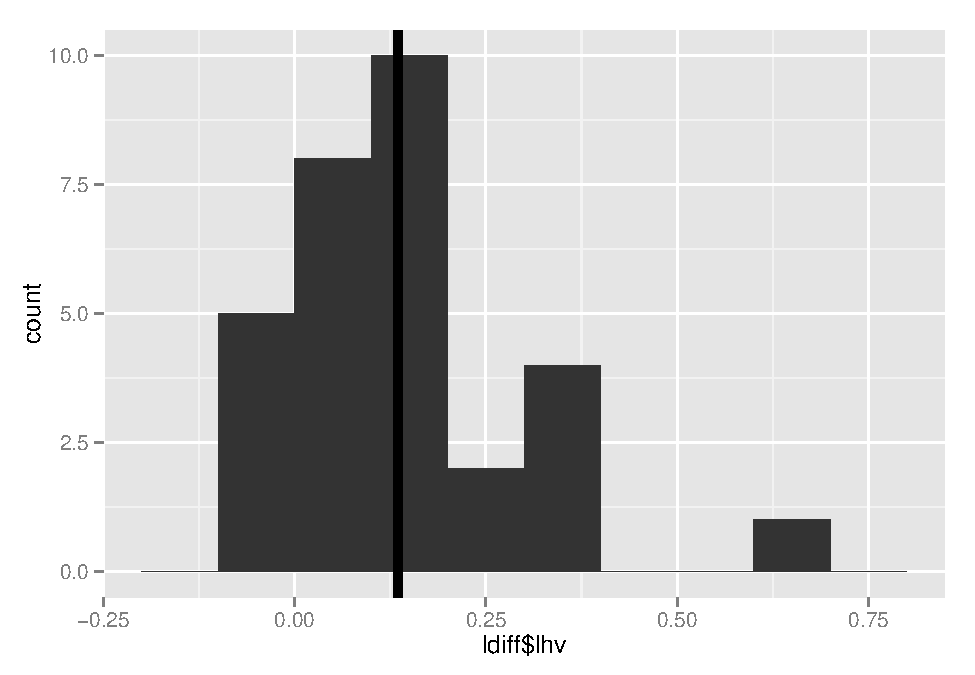
\includegraphics{ExtraFigs_files/figure-latex/ttestovgsps-1.pdf}

\begin{Shaded}
\begin{Highlighting}[]
\KeywordTok{qplot}\NormalTok{(rdiff$rhv,}\DataTypeTok{binwidth=}\FloatTok{0.1}\NormalTok{)+}\KeywordTok{geom_vline}\NormalTok{(}\DataTypeTok{x=}\NormalTok{rd$estimate,}\DataTypeTok{size=}\DecValTok{2}\NormalTok{)}
\end{Highlighting}
\end{Shaded}

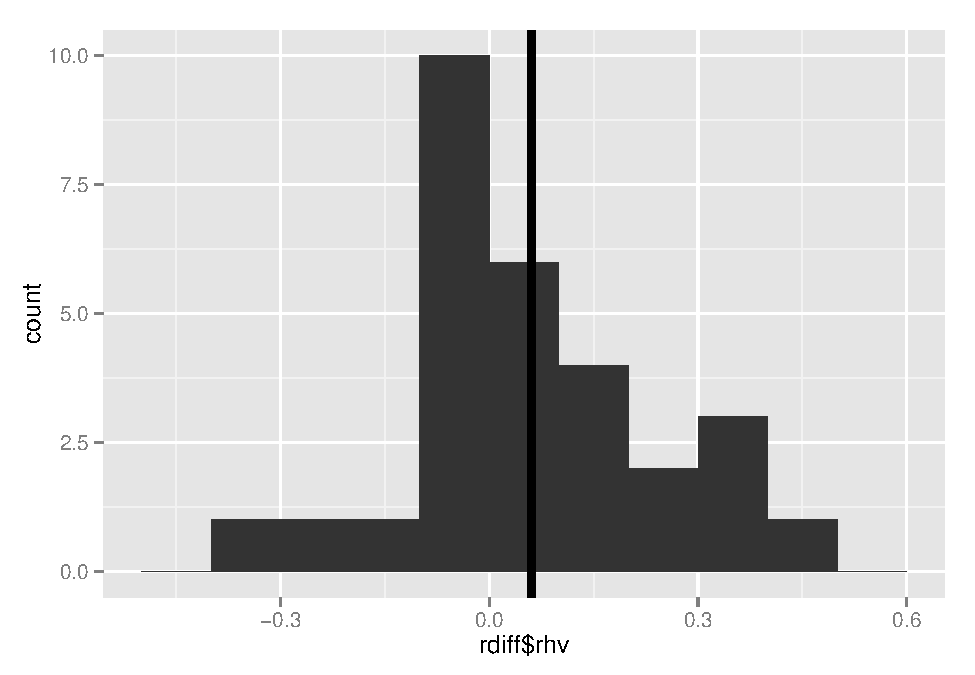
\includegraphics{ExtraFigs_files/figure-latex/ttestovgsps-2.pdf}

\begin{Shaded}
\begin{Highlighting}[]
\NormalTok{p<-}\KeywordTok{read.csv}\NormalTok{(}\StringTok{'~/MATLAB/NeurophysNRG/peakAnalysis.csv'}\NormalTok{,}\DataTypeTok{na.strings=}\StringTok{"NaN"}\NormalTok{)}
\KeywordTok{source}\NormalTok{(}\StringTok{'~/MATLAB/NeurophysNRG/RCode/StatSmoothFunc.R'}\NormalTok{)}
\KeywordTok{qplot}\NormalTok{(head_peak,maxsdf*}\DecValTok{1400}\NormalTok{,}\DataTypeTok{data=}\KeywordTok{subset}\NormalTok{(p,head_peak>}\DecValTok{0}\NormalTok{))+}
\StringTok{  }\KeywordTok{facet_wrap}\NormalTok{(~Neuron,}\DataTypeTok{ncol=}\DecValTok{2}\NormalTok{)+}
\StringTok{  }\KeywordTok{stat_smooth_func}\NormalTok{(}\DataTypeTok{method=}\StringTok{'lm'}\NormalTok{,}\DataTypeTok{geom=}\StringTok{'text'}\NormalTok{,}\DataTypeTok{parse=}\OtherTok{TRUE}\NormalTok{,}\DataTypeTok{hjust=}\DecValTok{0}\NormalTok{)+}\KeywordTok{stat_smooth}\NormalTok{(}\DataTypeTok{method=}\StringTok{'lm'}\NormalTok{)}
\end{Highlighting}
\end{Shaded}

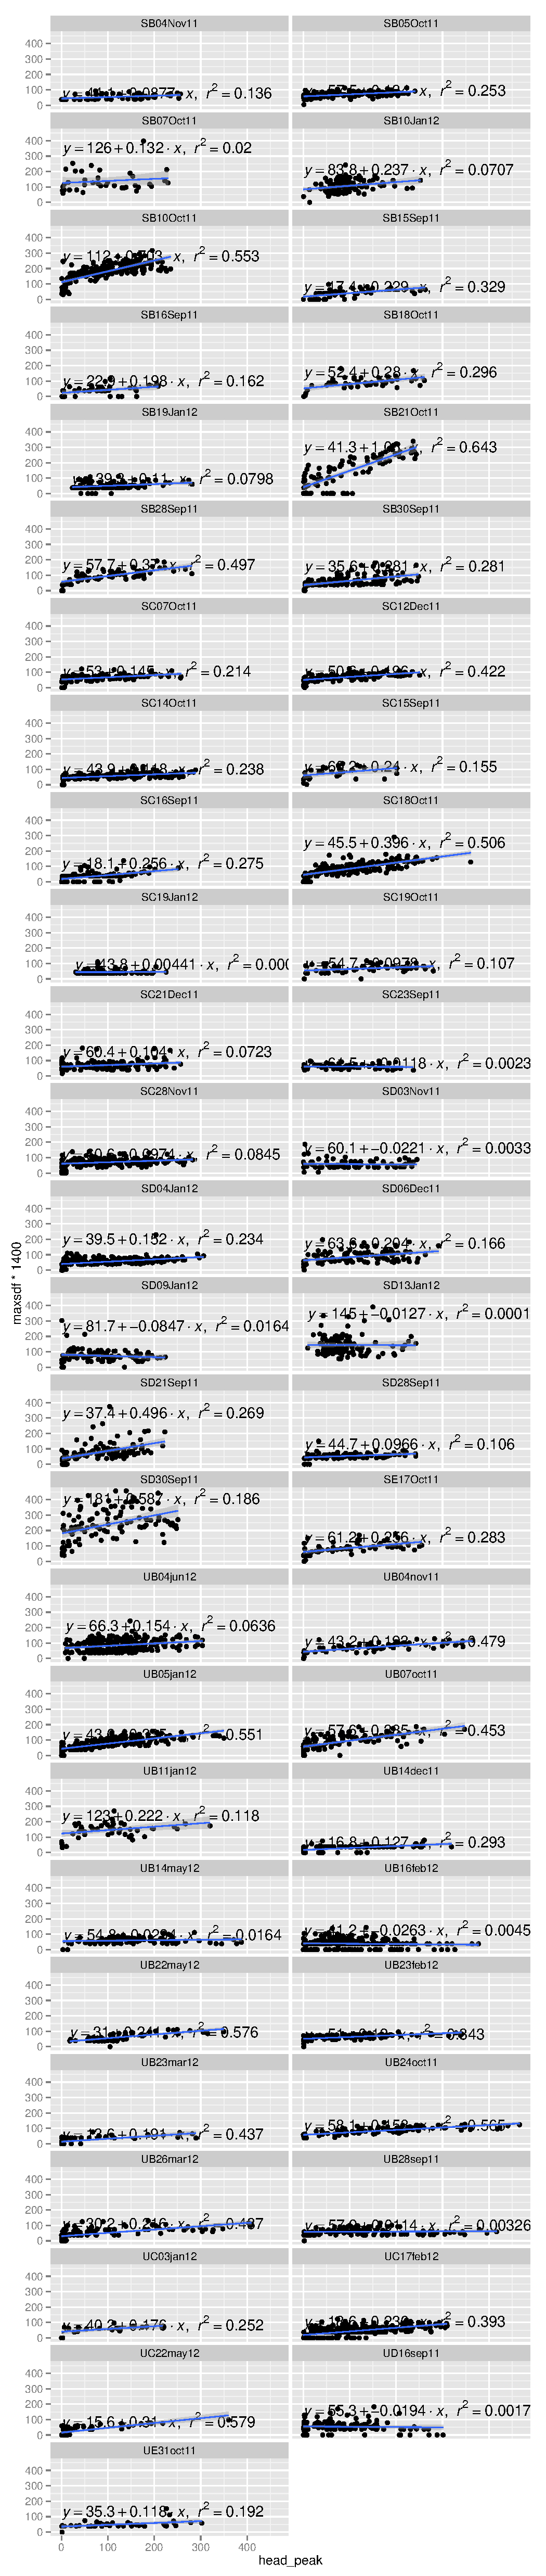
\includegraphics{ExtraFigs_files/figure-latex/peakAnalysis-1.pdf}

\begin{Shaded}
\begin{Highlighting}[]
\NormalTok{p$isgs<-}\KeywordTok{as.factor}\NormalTok{(p$isgs)}
\NormalTok{p %>%}
\StringTok{  }\KeywordTok{group_by}\NormalTok{(Neuron) %>%}
\StringTok{  }\KeywordTok{do}\NormalTok{(}\DataTypeTok{p.right=}\KeywordTok{summary}\NormalTok{(}\KeywordTok{lm}\NormalTok{(maxsdf ~}\StringTok{ }\NormalTok{head_peak,}\DataTypeTok{data=}\KeywordTok{filter}\NormalTok{(.,head_peak>}\DecValTok{20}\NormalTok{)))$coefficients[}\DecValTok{8}\NormalTok{],}
     \DataTypeTok{p.left=}\KeywordTok{summary}\NormalTok{(}\KeywordTok{lm}\NormalTok{(maxsdf ~}\StringTok{ }\NormalTok{head_peak,}\DataTypeTok{data=}\KeywordTok{filter}\NormalTok{(.,head_peak<}\StringTok{ }\NormalTok{-}\DecValTok{20}\NormalTok{)))$coefficients[}\DecValTok{8}\NormalTok{],}
     \DataTypeTok{p.left.slope=}
       \KeywordTok{summary}\NormalTok{(}\KeywordTok{lm}\NormalTok{(maxsdf ~}\StringTok{ }\NormalTok{head_peak*isgs,}\DataTypeTok{data=}\KeywordTok{filter}\NormalTok{(.,head_peak<}\StringTok{ }\NormalTok{-}\DecValTok{20}\NormalTok{)))$coefficients[}\DecValTok{16}\NormalTok{],}
     \DataTypeTok{p.left.int=}
       \KeywordTok{summary}\NormalTok{(}\KeywordTok{lm}\NormalTok{(maxsdf ~}\StringTok{ }\NormalTok{head_peak*isgs,}\DataTypeTok{data=}\KeywordTok{filter}\NormalTok{(.,head_peak<}\StringTok{ }\NormalTok{-}\DecValTok{20}\NormalTok{)))$coefficients[}\DecValTok{15}\NormalTok{],}
     \DataTypeTok{p.right.slope=}
       \KeywordTok{summary}\NormalTok{(}\KeywordTok{lm}\NormalTok{(maxsdf ~}\StringTok{ }\NormalTok{head_peak*isgs,}\DataTypeTok{data=}\KeywordTok{filter}\NormalTok{(.,head_peak>}\DecValTok{20}\NormalTok{)))$coefficients[}\DecValTok{16}\NormalTok{],}
     \DataTypeTok{p.right.int=}
       \KeywordTok{summary}\NormalTok{(}\KeywordTok{lm}\NormalTok{(maxsdf ~}\StringTok{ }\NormalTok{head_peak*isgs,}\DataTypeTok{data=}\KeywordTok{filter}\NormalTok{(.,head_peak>}\DecValTok{20}\NormalTok{)))$coefficients[}\DecValTok{15}\NormalTok{]) ->}
\StringTok{  }\NormalTok{mm}

\NormalTok{pp<-}\KeywordTok{merge}\NormalTok{(mm,p,}\DataTypeTok{by=}\StringTok{"Neuron"}\NormalTok{)}

\KeywordTok{qplot}\NormalTok{(head_peak,maxsdf*}\DecValTok{1400}\NormalTok{,}\DataTypeTok{col=}\NormalTok{isgs,}\DataTypeTok{data=}\KeywordTok{filter}\NormalTok{(pp,head_peak>}\StringTok{ }\DecValTok{20}\NormalTok{,p.right<}\FloatTok{0.001}\NormalTok{,p.right.slope<}\FloatTok{0.001} \NormalTok{|}\StringTok{ }\NormalTok{p.right.int<}\FloatTok{0.001}\NormalTok{))+}\KeywordTok{facet_wrap}\NormalTok{(~Neuron,}\DataTypeTok{ncol=}\DecValTok{3}\NormalTok{)+}\KeywordTok{stat_smooth}\NormalTok{(}\DataTypeTok{method=}\StringTok{'lm'}\NormalTok{)+}\KeywordTok{stat_smooth_func}\NormalTok{(}\DataTypeTok{method=}\StringTok{'lm'}\NormalTok{,}\DataTypeTok{geom=}\StringTok{'text'}\NormalTok{,}\DataTypeTok{parse=}\OtherTok{TRUE}\NormalTok{,}\DataTypeTok{hjust=}\DecValTok{0}\NormalTok{)}
\end{Highlighting}
\end{Shaded}

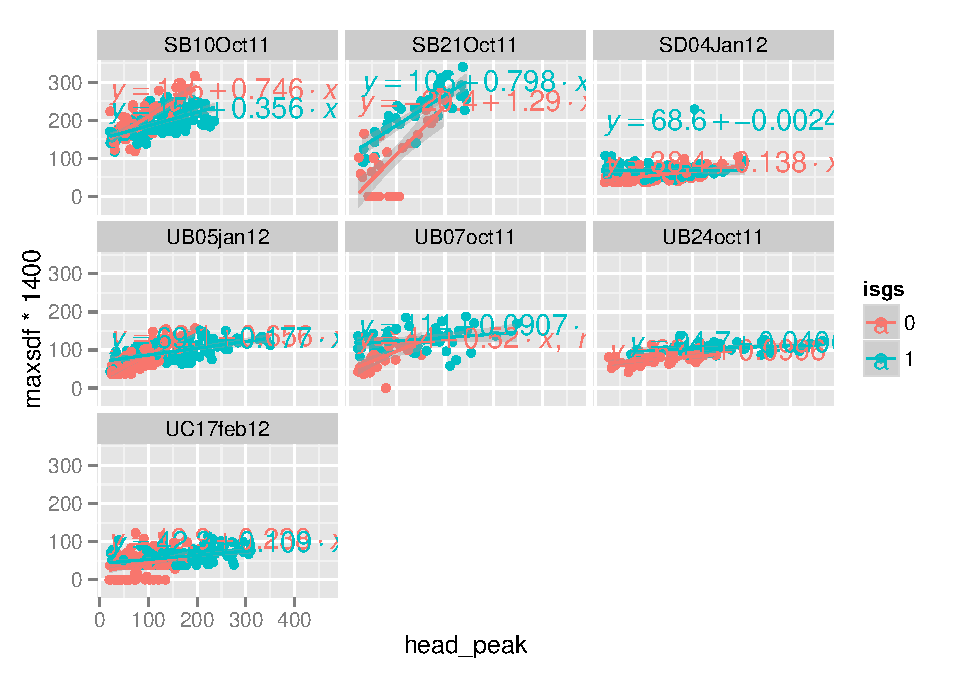
\includegraphics{ExtraFigs_files/figure-latex/gspsAnalysis-1.pdf}

\begin{Shaded}
\begin{Highlighting}[]
\KeywordTok{qplot}\NormalTok{(head_peak,maxsdf*}\DecValTok{1400}\NormalTok{,}\DataTypeTok{col=}\NormalTok{isgs,}\DataTypeTok{data=}\KeywordTok{filter}\NormalTok{(pp,head_peak<}\StringTok{ }\NormalTok{-}\DecValTok{20}\NormalTok{,p.left<}\FloatTok{0.001}\NormalTok{,p.left.slope<}\FloatTok{0.001} \NormalTok{|}\StringTok{ }\NormalTok{p.left.int<}\FloatTok{0.001}\NormalTok{))+}\KeywordTok{facet_wrap}\NormalTok{(~Neuron,}\DataTypeTok{ncol=}\DecValTok{3}\NormalTok{)+}\KeywordTok{stat_smooth}\NormalTok{(}\DataTypeTok{method=}\StringTok{'lm'}\NormalTok{)+}\KeywordTok{stat_smooth_func}\NormalTok{(}\DataTypeTok{method=}\StringTok{'lm'}\NormalTok{,}\DataTypeTok{geom=}\StringTok{'text'}\NormalTok{,}\DataTypeTok{parse=}\OtherTok{TRUE}\NormalTok{,}\DataTypeTok{hjust=}\DecValTok{0}\NormalTok{)}
\end{Highlighting}
\end{Shaded}

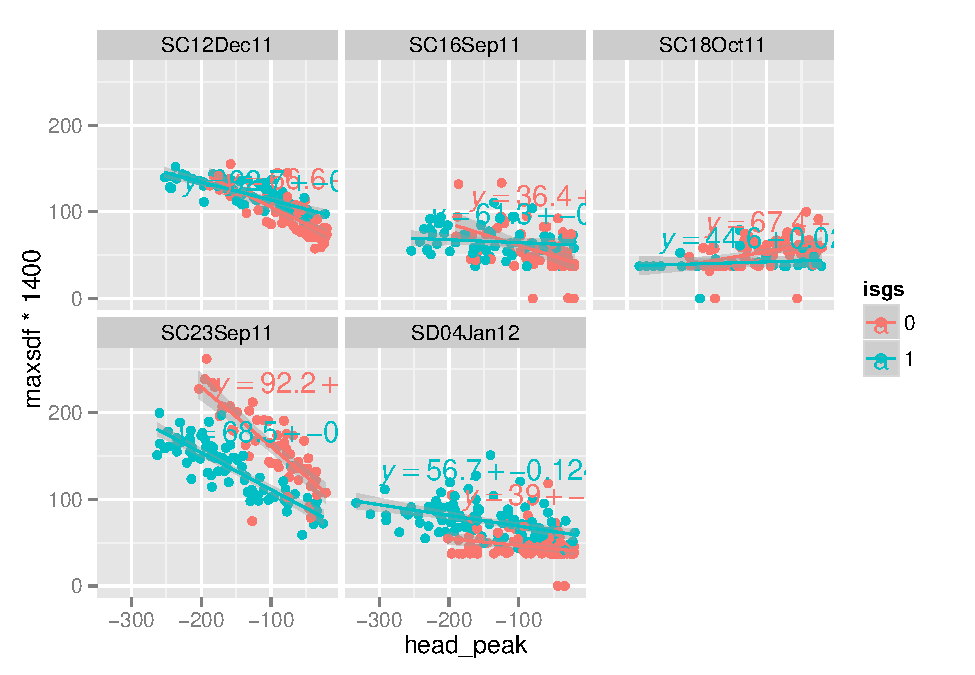
\includegraphics{ExtraFigs_files/figure-latex/gspsAnalysis-2.pdf}

\end{document}
